\documentclass[theme = light]{sprawozdanie}
\usepackage{lipsum}
\usepackage{enumitem}
\usepackage{adjustbox}
\usepackage{multirow}
\usepackage{placeins} % gives \FloatBarrier
\usepackage{hyperref}
\usepackage{booktabs}
% Beamer presentation requires 
%\usepackage{colortbl}


% ****************************************
%
    %TITLE PAGE
%\title{Termometr w dupie twoje starej}
\title{Wyznaczenie współczynnika siły \\[1mm] nośnej płata skośnego}
\class{Sprawozdanie z Laboratorium}
\author{ }
\deadline{28.10.2026}
\instructor{mgr inż. Konrad Gumowski}
%\instructor{dr inż. Tomasz Karolak}
%
%
%
    % MAIN
% ========================================
\begin{document}
\maketitle
%

\title{Wyznaczanie współczynnika siły nośnej płata skośnego }
\class{Bezzałogowe statki powietrzne}
%
% ----------------------------------------
%
    %SPIS TREŚCI
\tableofcontents\hfill\vfill
% ----------------------------------------
%
%% ZALADOWANIE FUNKCJI!!!!
% ===================================
% DŁUGOSCI DO JEDNEGO WYKRESY

\newlength{\singlePlotWidth}
\setlength{\singlePlotWidth}{\textwidth}

\newlength{\singleScreenshotWidth}
\setlength{\singleScreenshotWidth}{0.8\textwidth}

\newlength{\singlePhotoWidth}
\setlength{\singlePhotoWidth}{0.6\textwidth}

\newcommand{\newPlot}[3]{ 
        \begin{figure}[H]
        \centering
        \includegraphics[width = \singlePlotWidth]{wykresy/#1}
        \caption{#2}
        \label{fig:#3}
    \end{figure}
} 

\newcommand{\newScreenshot}[3]{ 
        \begin{figure}[H]
        \centering
        \includegraphics[width = \singlePlotWidth]{screenshots/#1}
        \caption{#2}
        \label{fig:#3}
    \end{figure}
} 

\newcommand{\newPhoto}[4]{ 
        \begin{figure}[H]
        \centering
        \includegraphics[width = #2]{zdjecia/#1}
        \caption{#3}
        \label{fig:#4}
    \end{figure}
} 

% #1 -> sciezka do obrazka
% #2 -> caption text

%\newcommand{\plot}[2]{
%    \begin{center}
%        \includegraphics[width=\singlePlotWidth]{#1}
%        \captionof{figure}{#2}
%    \end{center}
%}

\NewDocumentCommand{\plot}{m O{} O{\singlePlotWidth}}{%
  \begin{center}
    \includegraphics[width=#3]{#1}%
    \IfNoValueF{#2}{\captionof{figure}{#2}}%
  \end{center}%
}



% ===================================
% tabto skrotowo

\newcommand{\akapit}[0]{
\tabto{0.7cm}
}



% ====================================
% DŁUGOSCI DO OBRAZEK + TEKST W LINII
\newlength{\imagePageWidth}
\setlength{\imagePageWidth}{0.55\textwidth}

\newlength{\imageWidth}
\setlength{\imageWidth}{0.95\imagePageWidth}

\newlength{\myMargin}
\setlength{\myMargin}{0.025\textwidth}  % half of 0.05\textwidth


% Tworzy obrazek i obok daje tekst
% #1 -> sciezka obrazka
% #2 -> caption tekst
% #3 -> opis obok
\newcommand{\obrazTekst}[3]{
  \noindent
  \begin{minipage}[t]{\dimexpr\imagePageWidth - \myMargin\relax}
    \vspace{0pt}
    \centering
    \includegraphics[width=\imageWidth]{#1}
    \captionof{figure}{#2}
  \end{minipage}
  \hfill
  \begin{minipage}[t]{\dimexpr\textwidth - \imagePageWidth - \myMargin\relax}
    \vspace{0pt}
    #3
  \end{minipage}
}


% ----------------------------------------
%
\vfill

%
%
\newpage
% ------------
\section{Cel}
    \akapit Celem ćwiczenia jest zaznajomienie się z pomiarami wagowymi sił
aerodynamicznych oddziałujących na płat skrzydła modelu samolotu myśliwskiego i z interpretacją otrzymanych wyników.
% ------------
\section{Podstawy teoretyczne}
    \subsection{Parametry przepływu i własności fizyczne powietrza}
stanu gazu doskonale idealnego:
\begin{equation}
    \rho = \frac{p}{R \cdot T}
\end{equation}
gdzie:
\begin{itemize}
    \item $p$ - ciśnienie atmosferyczne,
    \item $R$ - stała gazowa dla powietrza $R \approx 287 \, \text{J}/(\text{kg}\cdot\text{K})$,
    \item $T$ - temperatura bezwzględna w kelwinach.
\end{itemize}

Znając gęstość powietrza oraz ciśnienie dynamiczne $q$ zmierzone w tunelu, prędkość przepływu niezakłóconego $V$ oblicza się, przekształcając wzór na ciśnienie dynamiczne:
\begin{equation}
    q = \frac{\rho V^2}{2} \implies V = \sqrt{\frac{2q}{\rho}}
\end{equation}

Z kolei kluczowym bezwymiarowym kryterium podobieństwa charakteryzującym opływ jest liczba Reynoldsa $Re$, definiowana za pomocą cięciwy profilu $c$, prędkości $V$ oraz lepkości kinematycznej powietrza $\nu$:
\begin{equation}
    Re = \frac{V \cdot c}{\nu}
\end{equation}

\subsection{Współczynnik siły nośnej}
W celu opisu wektora siły aerodynamicznej w układzie współrzędnych, rzut siły na oś prostopadłą do kierunku prędkości definiuje siłę nośną $P_z$. Aby uniezależnić wyniki od skali modelu i warunków pomiaru, siłę nośną opisuje się za pomocą bezwymiarowego współczynnika $C_z$:
\begin{equation}
    C_z = \frac{P_z}{\frac{\rho V^2}{2}S} = \frac{P_z}{qS}
\end{equation}
gdzie $S$ oznacza powierzchnię odniesienia. Dla ustalonej wartości liczby Reynoldsa współczynnik ten zależy wyłącznie od kąta natarcia $\alpha$.

% ------------
\section{Stanowisko pomiarowe}
    \akapit Badania przeprowadzono w tunelu aerodynamicznym wyposażonym w wagę aerodynamiczną Witoszyńskiego (typu JAW). Badany model zawieszony jest pionowo na napiętych drutach wewnątrz obrotowej ramy, której kąt natarcia można regulować w zakresie ±30° za pomocą samohamownej przekładni ślimakowej (odczyt kąta odbywa się ze skali na rurze wagi lub za pomocą przetwornika potencjometrycznego). Konstrukcja stanowiska umożliwia oddzielny (sekwencyjny) pomiar trzech składowych aerodynamicznych: siły nośnej, siły oporu oraz momentu pochylającego $M_yo$. Wybór mierzonej wielkości realizowany jest poprzez zablokowanie odpowiedniej pary sworzni $(S_z; S_x; S_m)$ i zwolnienie pozostałych, co nadaje ramie swobodę obrotu względem wybranej z trzech wzajemnie prostopadłych osi. Obciążenia z modelu przekazywane są przez układ drutów, ramę i dźwignie dwuramienne na tensometryczny przetwornik siły oraz połączoną z nim równolegle wagę szalkową służącą do wzorcowania układu. 

\akapit Badania przeprowadzono w tunelu aerodynamicznym, choć stanowisko to jest bazowo wyposażone w klasyczną wagę aerodynamiczną Witoszyńskiego (typu JAW), w trakcie realizowanego ćwiczenia zastosowano zmodyfikowany, zautomatyzowany układ mocowania i pomiaru. Zamiast tradycyjnego podwieszenia modelu na drutach, do obrotowej ramy wagi wykorzystano tzw. żądło (odpowiednio wygięty wysięgnik prętowy), na którego końcu osadzono badany model samolotu odrzutowego. Do wyznaczenia obciążeń aerodynamicznych wykorzystano, wewnętrzną wagę tensometryczną umieszczoną bezpośrednio wewnątrz modelu, co wyeliminowało konieczność stosowania zewnętrznego układu dźwigni i drutów. Zmiana kąta natarcia (realizowana poprzez obrót ramy z żądłem za pomocą przekładni napędzanej silnikiem elektrycznym) oraz akwizycja danych pomiarowych z czujnika odbywały się zdalnie z poziomu komputera wyposażonego w dedykowane oprogramowanie pomiarowe. 

% ------------
\section{Przebieg ćwiczenia}
    \akapit Zgodnie z instrukcją wykonano następujące czynności:
\begin{enumerate}[itemsep = 1mm, parsep = 1mm, topsep = 3mm, partopsep = 0mm, leftmargin = 1.4cm]
    \item Wybrano parametry pracy tunelu aerodynamicznego i ustawiono zakres kątów dla których miał się odbyć pomiar
    \item Uruchomiono program pomiarów
    \item Wyniki sczytano na pendrive 
\end{enumerate}

\akapit Następnie dokonano niezbędnych obliczeń w celu otrzymania pożądanych charakterystyk płata w funkcji kąta natarcia. Wyniki przedstawiono w sekcji \ref{sec:Wyniki}. Obliczeń dokonano z użyciem środowiska Matlab\footnote{i GNU Octave, ale to kolega ma zboczenie takie}.
% ------------
\newpage
\section{Wyniki}
    \label{sec:Wyniki}

\akapit Wyniki pomiarowe przedstawiono w poniższej tabeli. Posłużyły one do późniejszego obliczenia odpowiednich charakterystyk.

\begin{table}[H]%[htbp]
    \centering
    \caption{Zestawienie wyników pomiarów aerodynamicznych}
    \label{tab:pomiary}
    \vspace{0.6em}
    \small
    \setlength{\tabcolsep}{10pt}
    \renewcommand{\arraystretch}{1.12}
    \begin{tabular}{r r r r r r r r}
        \toprule
        $\alpha$ & $\beta$ & $N$ & $m$ & $T$ & $C$ & $n$ & $l$ \\
        \midrule
        -2.903 & 0.000 & -3.635 &  0.069 &  0.495 &  0.384 & -0.008 & -0.034 \\
        -2.000 & 0.000 & -2.908 &  0.054 &  0.524 &  0.363 & -0.009 & -0.034 \\
        -0.000 & 0.000 & -1.352 &  0.025 &  0.550 &  0.288 & -0.013 & -0.041 \\
         2.000 & 0.000 &  0.375 &  0.006 &  0.539 &  0.258 & -0.017 & -0.053 \\
         4.000 & 0.000 &  2.053 & -0.011 &  0.480 &  0.227 & -0.022 & -0.061 \\
         6.000 & 0.000 &  3.749 & -0.029 &  0.400 &  0.164 & -0.023 & -0.069 \\
         8.000 & 0.000 &  5.528 & -0.048 &  0.358 &  0.113 & -0.026 & -0.078 \\
        10.000 & 0.000 &  7.093 & -0.063 &  0.260 &  0.085 & -0.027 & -0.081 \\
        12.000 & 0.000 &  8.627 & -0.071 &  0.186 &  0.069 & -0.028 & -0.084 \\
        14.000 & 0.000 & 10.135 & -0.064 &  0.115 &  0.032 & -0.029 & -0.084 \\
        16.000 & 0.000 & 11.627 & -0.067 &  0.034 & -0.019 & -0.030 & -0.095 \\
        18.000 & 0.000 & 13.175 & -0.073 & -0.059 & -0.058 & -0.030 & -0.091 \\
        20.000 & 0.000 & 14.358 & -0.064 & -0.133 & -0.137 & -0.025 & -0.084 \\
        22.000 & 0.000 & 15.311 & -0.043 & -0.161 & -0.301 & -0.006 & -0.067 \\
        24.000 & 0.000 & 16.324 & -0.019 & -0.176 & -0.469 &  0.009 & -0.058 \\
        26.000 & 0.000 & 17.364 &  0.026 & -0.180 & -0.460 &  0.005 & -0.069 \\
        28.000 & 0.000 & 18.429 &  0.055 & -0.179 & -0.433 &  0.006 & -0.051 \\
        30.000 & 0.000 & 19.029 &  0.162 & -0.022 &  0.111 &  0.112 &  0.035 \\
        32.000 & 0.000 & 19.987 &  0.161 & -0.065 &  0.089 &  0.123 &  0.013 \\
        33.999 & 0.000 & 20.140 &  0.187 &  0.161 &  0.057 &  0.036 & -0.061 \\
        36.000 & 0.000 & 21.236 &  0.181 &  0.076 &  0.143 &  0.043 & -0.054 \\
        37.999 & 0.000 & 22.269 &  0.170 & -0.009 &  0.167 &  0.039 & -0.049 \\
        39.999 & 0.000 & 22.978 &  0.154 & -0.074 &  0.107 &  0.025 & -0.057 \\
        \bottomrule
    \end{tabular}
\end{table}

\newpage
\begin{figure}[H]
    \centering
    %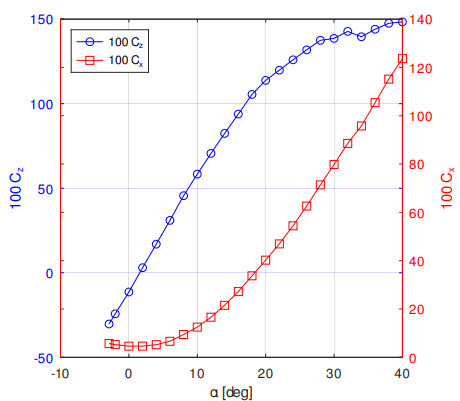
\includegraphics[width=0.5\linewidth]{zdjecia/CzCx.png}
    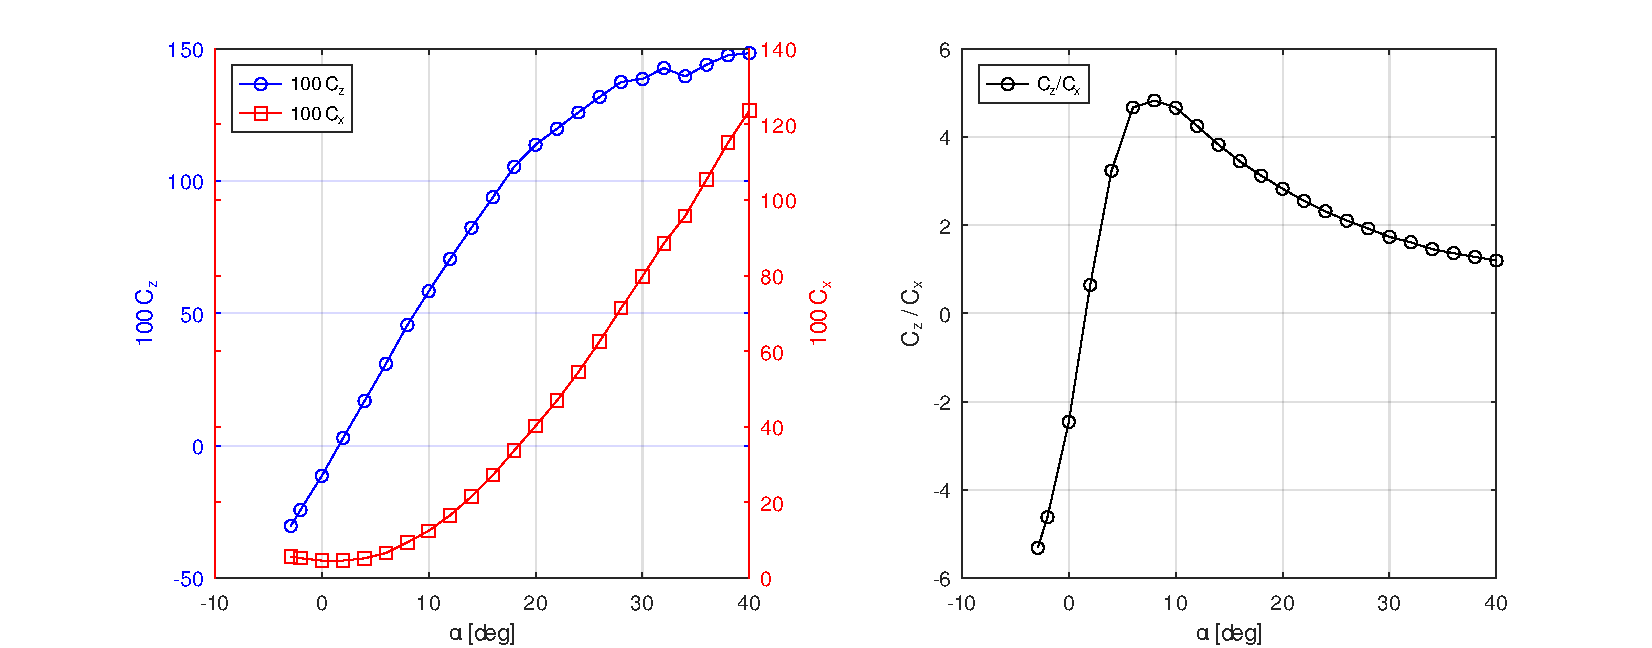
\includegraphics[width = 0.95\linewidth]{zdjecia/cz_cx_ld.pdf}
    \caption{Zależność współczynników $C_x$, $C_z$ i doskonałości $\frac{C_x}{C_z}$ od kąta natarcia skrzydła}
    \label{fig:cxcz}
\end{figure}

\begin{figure}[H]
    \centering
    %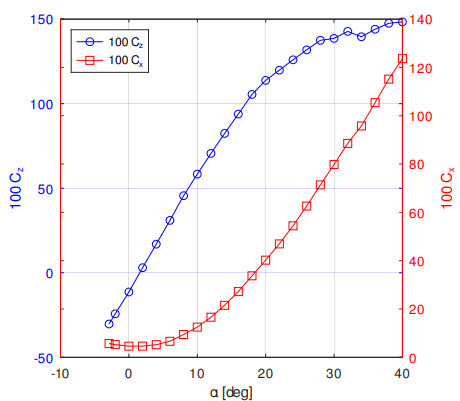
\includegraphics[width=0.5\linewidth]{zdjecia/CzCx.png}
    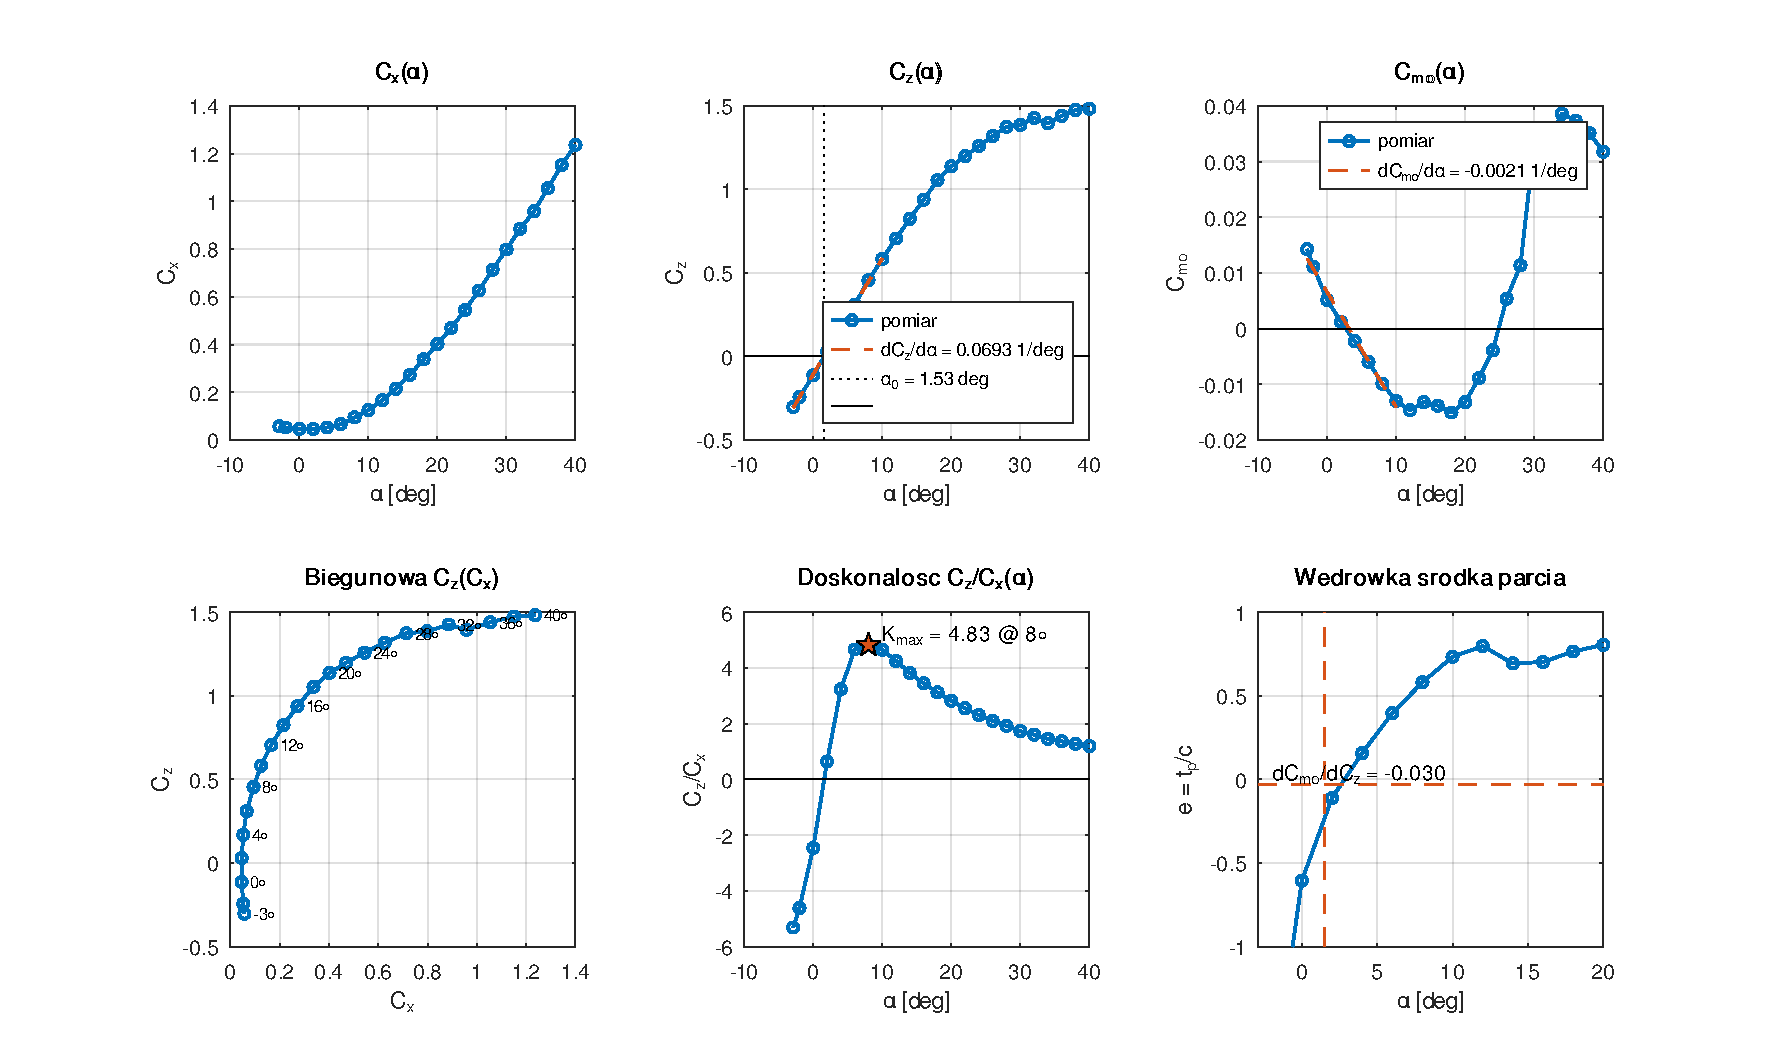
\includegraphics[width = 0.95\linewidth]{zdjecia/charakterystyki.pdf}
    \caption{Zestawienie charakterystyk na osobnych wykresach\protect\footnotemark}
    \label{fig:charakterystyki}
\end{figure}
\footnotetext{Wykres wędrówki środka parcia prawdopodobnie jest błędny}

\vfill
% ------------
\section{Wnioski}
    \begin{enumerate}[itemsep = 4mm, parsep = 3mm, topsep = 5mm, partopsep = 2mm, leftmargin = 0.5cm]

\item \textbf{Analiza wykresu Cx Cz w fukncji kąta natarcia $\alpha$} 
    \akapit Na podstawie sporządzonego wykresu Cx i Cz od $\alpha$ zauważyć można że uzyskane w ramach laboratorium charakterystyki płata są zgodne z teoretycznymi przewidywaniami. Wartość współczynnika Cx odpowiadającego za siłę oporu jest zgodnie z intuicją zawsze dodatnia. Współczynnik Cz, powiązany z siłą nośną, natomiast przecina oś OX wykresu i przyjmuje ujemne wartości dla ujemnych kątów natarcia co również jest zgodne z przewidywaniami dla standardowych ( nie samostatecznych ) profili płatów. Ponadto tak jak teoretycznie zakładano uzyskany wykres Cx jest praktycznie liniowy dla małych kątów natarcia tzn poniżej ok 20 stopni.

\item \textbf{Analiza wykresu doskonałości}
   \akapit Wykres $\frac{C_x}{C_z}$ od kąta natarcia zwany również wykresem doskonałości, również pokrywa się z oczekiwaniami, posiada max w okolicy 8 stopni kąta natarcia, co oznacza że jest najbardziej wydajny aerodynamicznie dla takiego ustroju lotu.

\item \textbf{Podsumowanie}
    \akapit Uzyskane wyniki pokrywają się z przewidywaniami teoretycznymi oraz z przedstawionymi na laboratoriach historycznymi pomiarami innych profili płatów. Taka powtarzalność oraz przewidywalność wyników, nawet pomimo różnych metod obróbki danych - kiedyś ręcznego wyrównywania wag szalkowych, a dzisiaj cyfrowej analizy danych, świadczy o dużej wartości metody pomiarów z użyciem wagi aerodynamicznej nawet w epoce oprogramowania CFD.
\end{enumerate}
%

\end{document}

